\documentclass[12pt]{article}
\usepackage[a4paper, total={7.5in, 11in}]{geometry}
%\usepackage{array}
\usepackage{graphicx, subfig, wrapfig, fancyhdr, lastpage, multicol ,color,arydshln,makecell}
\newcommand\headerMe[2]{\noindent{}#1\hfill#2}
\usepackage[mathscr]{euscript}
\usepackage{tabularray}

\setlength{\columnseprule}{1pt}
\def\columnseprulecolor{\color{blue}}


\pagestyle{fancy}
\fancyhf{}

\cfoot{ \vspace{-0.8cm}\em{Page \thepage \hspace{1pt} / \pageref{LastPage}}}
\begin{document}

\headerMe{Royaume du Maroc}{année scolaire \emph{2023-2024}}\\
\headerMe{Ministère de l'Éducation nationale, }{  Professeur :\emph{Zakaria Haouzan}}\\
\headerMe{du Préscolaire et des Sports}{Établissement : \emph{Lycée SKHOR qualifiant}}\\
\vspace{-1cm}
\begin{center}
Devoir Surveillé  N°1 \\
    2ème année baccalauréat Sciences physiques\\
Durée 2h00
\\
    \vspace{.2cm}
\hrulefill
\Large{Chimie 7pts - 55min}
\hrulefill\\

    %\emph{Les deux parties sont indépendantes}
\end{center}
%end Headerss------------------------
%__________________Chimie ______________________-
%%%%%%%+_+_+_+_+_+_+_+_+_Partie1

 \section*{Suivi temporel d’une transformation chimique par manométrie\dotfill(7pts) }
 \begin{wrapfigure}{r}{0.360\textwidth}

	\vspace{-1.2cm}
\begin{center}
  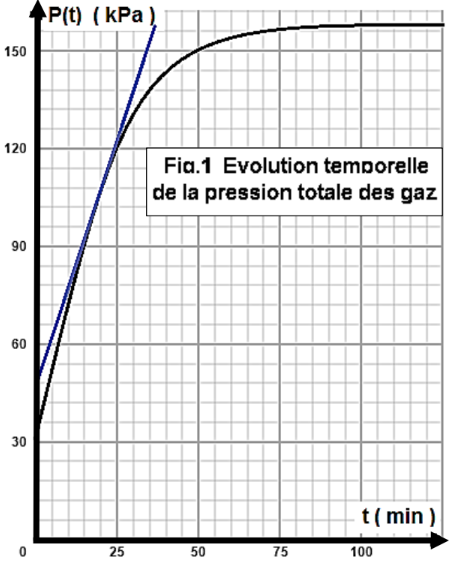
\includegraphics[width=0.340\textwidth]{./img/fig00.png}
\end{center}
\end{wrapfigure}

Le monoxyde de carbone $CO$ forme avec le fer solide un composé de formule $Fe(CO)_5$ appelé pentacarbonylfer.
À $200$ °C $= 473 K$, dans l'obscurité, le pentacarbonylfer gazeux se décompose lentement mais totalement en fer solide
et monoxyde de carbone gazeux selon l’équation suivante :

$${Fe(CO)_5}_{(g)} \rightarrow  Fe_{(s)}  + 5 CO_{(g)}$$

On supposera se placer dans un réacteur fermé de volume $V$=$250mL$ et préalablement vidé de l’air. On y enferme
une quantité $n_0 = 2,0 mmol$ de pentacarbonylfer puis on chauffe à $T = 473 K$. On enregistre la pression totale $P(t)$
dans ce réacteur en fonction du temps. Les gaz sont assimilés à des gaz parfaits et on prendra $R = 8,31 SI$.

\begin{tabular}{c|l}
	0,5  & \makecell[l]{ \textbf{1. }Un gaz parfait est un modèle thermodynamique \\décrivant le comportement des gaz réels à\\basse pression. Il
est régi par une équation dite \\équation d’état des gaz parfaits.\\Ecrire cette équation puis Déduire l’unité de R. }\\


	0,25  & \makecell[l]{ \textbf{2. }Vérifier que $P_0$ la pression à l’état initial vaut : $P_0 = 31,4 kPa$.}\\


	0,5  & \makecell[l]{ \textbf{3. }Dresser le tableau d’avancement de cette réaction. }\\
	
	0,5  & \makecell[l]{ \textbf{4. }Montrer que l’avancement $x(t)$ est relié à la pression totale $P(t)$ par la relation suivante: \\$x(t)$ = $\frac{V}{4.R.T}.P(t)$ - $\frac{n_0}{4}$ }\\


	1  & \makecell[l]{ \textbf{5. }Montrer que l’expression de la vitesse volumique, en $mol.L^{-1}.min^{-1}$en fonction de P(t) \\s’écrit sous la forme : $v = 6,63.10^{-5}. \frac{dP}{dt}$ }\\ 

	0,5 & \makecell[l]{ \textbf{6. }Définir ce que c’est qu’un facteur cinétique. }\\
	
	0,5    & \makecell[l]{ \textbf{7. }Comment varie cette vitesse volumique ? Quel est le facteur cinétique responsable de\\cette variation ? }\\
	
	0,5 & \makecell[l]{ \textbf{8. }Déterminer graphiquement $v_{20}$ la valeur de la vitesse volumique de la réaction à\\la date t = 20 min.}\\
	
	0,75 & \makecell[l]{ \textbf{9. }Calculer la composition du système à l’instant $t = 25s$.}\\
	
	1 & \makecell[l]{\textbf{10. }Montre que la pression à la date $t_{1/2}$ s’exprime sous la forme : $P(t_{1/2}) = \frac{P_0 + P_{max}}{2}$ puis déduire \\la valeur de $t_{1/2}$.}\\
	
	1 & \makecell[l]{ \textbf{11. }On refait l’expérience précédente mais avec une quantité $n_1= 3.n_0$ de pentacarbonylfer dans\\le même volume V.
représenter, l’allure de la nouvelle courbe représentant P(t) en bleu.\\Si on porte ce nouveau mélange réactionnel
à la température de 208°C, tracer sur le même graphe\\la nouvelle courbe en vert.(Recopier le repère ci-dessous). }\\
\end{tabular}

\begin{center}
	.
\end{center}
\vspace{1cm}

    \emph{Les  parties sont indépendantes}
%\hrulefill
%\Large{Physique 13pts/78min}
%\hrulefill\\
\begin{center}
    %\vspace{.60cm}
\hrulefill
\Large{Physique 13pts - 65min}
\hrulefill\\
    \emph{Les  parties sont indépendantes}
\end{center}

\vspace{-1cm}
\section*{Partie 1 :  le mouvement des vagues .......(4pts)}
\vspace{-0.4cm}

\begin{wrapfigure}[2]{r}{0.43\textwidth}

  \begin{center}
	  \vspace{-2cm}
	  \hspace{2cm}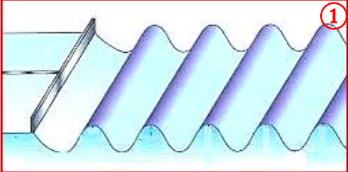
\includegraphics[width=0.19\textwidth]{./img/fig02.png}
	  \hspace{2cm}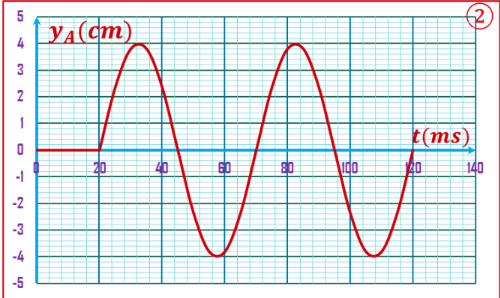
\includegraphics[width=0.43\textwidth]{./img/fig03.png}
  \end{center}
\end{wrapfigure}

Sur une cuve à ondes, on crée à un instant $t_0 = 0s$ des ondes
mécaniques rectilignes sinusoïdales , grâce à une réglette plane
menue d’un vibreur . Ces ondes se propagent sur la \\surface d’eau
sans atténuation et sans réflexion. La figure (1)\\
La figure 2 représente l’évolution temporelle de l’élongation \\d’un
point A situé a une distance $d = 4cm$ \\de la lame vibrante.


\begin{tabular}{c|l}

 0,5 & \makecell[l]{\textbf{1. } L’onde étudiée est-elle longitudinale ou \\transversale ? Justifier.}\\
 1 & \makecell[l]{\textbf{2. }Calculer V, la vitesse de propagation de ces ondes.}\\
 
 1 & \makecell[l]{\textbf{3. }Calculer la longueur d’onde à la surface de l’eau.}\\

 1   & \makecell[l]{\textbf{4. }On considère un point B de la surface de l’eau\\
tel que $AB = 10cm$.Comparer les états vibratoires des points A et B }\\

 0,5   & \makecell[l]{\textbf{5. }Sur la figure 2 tracer l’allure de l’élongation du
	B sur l’intervalle [0ms, 120ms].}\\

\end{tabular}


\section*{Partie 2 : Étude du phénomène ondulatoire. \dotfill(4pts) }
\begin{wrapfigure}[6]{r}{0.29\textwidth}
  \begin{center}
	  \vspace{-1.5cm}
	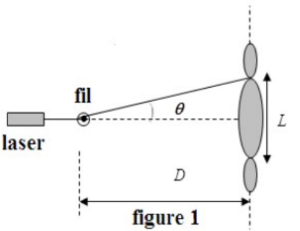
\includegraphics[width=0.29\textwidth]{./img/diff.png}
  \end{center}
\end{wrapfigure}


On réalise une expérience en utilisant un LASER, un fil de diamètre a et un écran. Le dispositif est
représenté ci-dessous (figure 1) :
Les mesures de diamètre du fil a, de la distance du fil à l’écran D
et de la largeur de la tache lumineuse centrale L conduisent
aux résultats suivants : $a = 0,200mm$ et $D=2,00m$ ; $L=12,6mm$.

\begin{tabular}{c|l}
	1 & \makecell[l]{\textbf{1. }Quel est le nom du phénomène observé et déduire la nature de \\la lumière  ?}\\
	0,5	&\makecell[l]{\textbf{2. } a l’aide de la figure 1, Etablir la relation entre $\theta$, L et D\\on supposera $\theta$ est suffisamment petit pour considérer $tan(\theta) = \theta$ avec $\theta$ exprimé en radian.}\\
		0,5& \makecell[l]{\textbf{3. }En utilisant les résultats des mesures, calculer la valeur de l’angle $\theta$ en radians.}\\

	0,5 &\makecell[l]{\textbf{4. }Donner la relation qui lie les grandeurs $\theta$ (écart angulaire), $\lambda$ (longueur d’onde de la
lumière)\\et a (diamètre du fils). Préciser les unités (dans le système international) respectives de ces\\grandeurs physiques.}\\
	0,5 &\makecell[l]{\textbf{5. }Calculer la valeur de la longueur d’onde $\lambda$. Est-ce qu’elle appartient au domaine visible?\\justifier.}\\

	1 &\makecell[l]{\textbf{6. }Comment différencier expérimentalement une lumière monochromatique d’une lumière
\\polychromatique
	}\\
\end{tabular}

\section*{Partie 2 :  Dispersion d’une onde lumineuse par un prisme\dotfill(5pts) }
\begin{wrapfigure}[6]{r}{0.3\textwidth}
  \begin{center}
	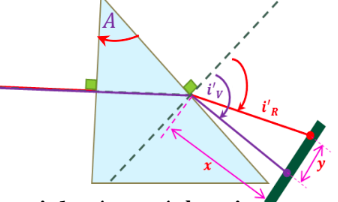
\includegraphics[width=0.3\textwidth]{./img/prisme.png}
  \end{center}
\end{wrapfigure}

Un faisceau lumineux composé de deux radiations rouge et
violette arrive orthogonalement (i = 0°) sur une face d’un
prisme en verre , la figure ci-contre .

\begin{tabular}{c|l}
	2 &\makecell[l]{\textbf{1. }Calculer les angles de déviations $D_R$ $(i'_R)$ et $D_V$ ($i'_v$) .}\\

	1 &\makecell[l]{\textbf{2. }On place à la distance x = 4cm un écran perpendiculaire sur \\le rayon violet émergé du prisme.\\
	Calculer la distance y entre la tache rouge et la tache violette sur l’écran .}\\

	1 &\makecell[l]{\textbf{3. }Que peut-on dire à propos du verre constituant le prisme}\\
	
	1 &\makecell[l]{\textbf{4. }Calculer la longueur d’onde du rayon rouge dans le prisme.}\\
\end{tabular}

\begin{center}
\begin{itemize}
	\item Les indices de réfraction du prisme pour les deux radiations: $n_V$=$1, 652$ et $n_R = 1, 618$  et $n_{air} = 1$	
	\item  La longueur d’onde du rayon rouge dans le vide $\lambda_{0R} = 768nm$ et L’angle du prisme $A =$ 35°

\end{itemize}

\end{center}

\end{document}
